\documentclass[10pt,a4paper]{article}
\usepackage[latin1]{inputenc}
\usepackage{amsmath}
\usepackage{amsfonts}
\usepackage{amssymb}
\usepackage{makeidx}
\usepackage[pdftex]{graphicx}
\author{Magni Nicol\'as, Purita Nicol\'as, Zemin Luciano R.  }
\title{Multitasker}
\begin{document}
\maketitle
\newpage
\tableofcontents
\clearpage

\section{Introducci\'on}
	\subsection{Objetivo}
		Se debe crear un sistema Operativo Multitarea, asignandoles a cada proceso un tiempo de ejecuci\'on. El multitasker corre directamente sobre memoria y montado sobre una base de un sistema monotarea. Para cargar el Sistema Operativo se utiliza el bootloader GRUB de Unix.
	\subsection{Enunciado}
Se desea implementar un Multitasker, cuyo objetivo  principal es asignar tiempo de ejecuci \'on a\ diferentes procesos en memoria. El sistema deber\'a ser implementado para plataformas Intel de 32 bits, utilizando el procesador en modo protegido. El multitasker debera ser preemptivo, es decir, cualquier tarea puede ser desalojada del microprocesador. El encargado de administrar el CPU es el scheduler el cual tomar\'a como base de tiempo la interrupci\'on de hardware INT8 correspondiente al timer tick, para realizar la asignaci\'on de tiempo ( time slot ).

	\subsection{Actividades}
		\begin{enumerate}	
			\item Se deber\'a elegir la forma en resguardar el contexto de cada tarea, se debera elejir entre las siguientes opciones
			\begin{itemize}
				\item Utilizar los TSS que provee el microprocesador Intel 386 
				\item Realizar una implementaci\'on propia de c\'odigo.
			\end{itemize}

			\item Se debera implementar dos tipos de scheduling distintos . Principalmente uno de ellos deber \'a considerar la prioridad de los procesos para asignar los slots de tiempo.

			\item El sistema deber\'a estar programado de manera que se diferencien los estados b\'asicos de Corriendo, Esperando y Listo. Por otra parte, cada proceso deber \'a tener un valor de prioridad entre 0 y 4 que indique la importancia del proceso.  Adem\'as se deber\'an demostrar el funcionamiento de los mismos con programas de prueba y se deber\'a poder corroborar el estado del proceso y el porcentaje de procesador que est\'a ocupando con la ayuda del comando top. Tambi\'en deber \'a haber un comando kill que permita matar procesos en ejecuci\'on. Tener en cuenta que kill debe matar tambi\'en a todos los hijos de ese proceso.


			\item Se debera poder tener al menos 4 terminales distintas y alternar entre ellas de manera similar a Linux.

			\item Se debera poder ejecutar diferentes tareas a trav\'es de comandos ingresados por teclado. La sintaxis de los comandos quedan a elecci\'on del desarrollador.

			\item El sistema debe tener la posibilidad de correr los mismos procesos tanto en foreground como en background. Para este ultimo se deber\'a utilizar el caracter \& al igual que en UNIX.

			\item El sistema debe tener un m\'odulo de administraci\'on de memoria mediante paginaci\'on para los procesos, el mismo se encargar\'a de lo siguiente:
			\begin{itemize}
				\item Cada proceso tendr\'a su stack propio en una p\'agina, a la cual solamente  \'el tendr\'a acceso. Cada proceso podr\'a leer y escribir libremente sobre esta p\'agina pero no p\'aginas de otros procesos.
				\item Los procesos no poseer\'an un heap propio, ya que est\'an corriendo sobre la misma zona de datos del SO.
				\item Ningu\'n proceso deber\'a leer o escribir directamente ninguna variable global del SO. En caso de que haya variables globales que est\'en pensadas para ser leidas por procesos usuario, deber\'an tener una funci\'on que las copie a una zona de heap propia al proceso, simulando un system call.
			\end{itemize}
		\end{enumerate}

\section{Material entregado}
	
\section{Lineamientos de desarrolo}

\section{Kernel}
	\subsection{Objetivo}
		El \textit{Kernel} es el encargado de levantar todo el sistema operativo.
	\subsection{Esquema general}
		La funci\'on principal del \textit{Kernel} es cargar en la IDT las rutinas de atenci\'on del teclado, del timer tick y las interrupciones de la \textit{int 80}, iniciar la paginaci\'on, iniciar el multitasker e inicializar las TTYs. Ademas de todas estas inicializaciones, tambien inicia el driver de video, el m\'odulo de shared memory, los sem\'aforos y por \'ultimo habilita las entradas del Pic que correspondan para el Timer Tick y la del Teclado. 
	\subsubsection{LLamadas a Sistema}
		Para inicializar cada m\'odulo se realiza una llamada a sistema, ya que en ese instante que esta inicializando no puede perder el procesador, por lo tanto todas estas funciones antes desabilitan las interrupciones. Toda funci\'on que hayamos considerado que no pueden perder la atenci\'on hacen una llamada a sistema.
	\subsubsection{Drivers y Perisf\'ericos}

\section{Paginacion}
	\subsection{Objetivo}
		El sistema operativo debe tener un m\'odulo de paginaci\'on, por lo tanto cada proceso debe tener asociado cierta cantidad de p\'aginas. Por consecuente se debe implementar la excepci\'on correspondiente a paginaci\'on ya que el m\'odulo de administraci\'on de memoria debe verificar que un proceso no utilize p\'aginas no asignadas a \'el. Todos los procesos comparten el heap, es decir que no existen variables globales dentro del sistema operativo y en el caso que se existiesen deben estar en el heap del kernel, por lo tanto si el proceso desea obtener algun valor de alguna variable debe simular un system call y copiar la variables al heap propio del proceso.
	\subsection{Modelo}
	\subsection{Esquema general}
		Como se implement\'o un m\'odulo de administraci\'on de memoria, se debio implemantar un \textit{malloc}. Un criterio tomado es que el kernel llama una sola vez al memory map donde obtiene todo su espacio kernel,en cambio el malloc llama reiteradas veces al memory map donde se asignan las p\'aginas asociadas al heap de ese proceso. Toda la informaci\'on de las p\'aginas asignadas se encuentran en la tabla de procesos.
	\subsection{Problemas y soluciones}
		Un gran problema que obtuvimos por medio de la paginaci\'on fue que no podiamos crear mas de 4 procesos en simult\'aneo, esto se produjo ya que luego de ver reiteradas veces el c\'odigo y no darnos cuenta cual era la cause del Page Fault, decidimos seguirlo desde c\'odigo Assembler donde pudimos encontrar la raz\'on por la que se lanzaba la excepci\'on y era porque el \textbf{CR2} tenia carada una direcci\'on de una p\'agina invalida por lo tanto no estaba presente y lanzaba Page Fault. El principal problema fue en el armado de los frames de las p\'aginas, donde el algoritmo no contemplaba un caso donde habia que dar de baja un frame, levantar otro y asi consecutivamente. Luego de una gran reestructuraci\'on de nuestro sistema se nos paso asignar los nuevos valores definidos en \textit{defs.h} para llevar a cabo la paginaci\'on, por lo tant retornaba direcciones no deseadas.
	\subsection{Limitaciones}
		Como no se utiliz\'o segmentacion de p\'aginas, el malloc siempre retornaba p\'aginas contiguas y no se almacenaba ningun registro sobre segmentos otorgados.

\section{File System} 
	\subsection{Modelado}
		Se implment\'o una simulaci\'on de un File System, pero unicamente teniendo los pseudoarchivos \textit{STDIN} y \textit{STDOUT}. Cada proceso tiene almacenado en su estructura estos pseudoarchivos.
	\subsection{Esquema general}
	\subsection{Problemas y soluciones}
	\subsection{Limitaciones}

\section{TTY}
	\subsection{Objetivo}
		Dado un numero maximo de tty's estas son creadas en la inicializaci\'on del  sistema. Estas almacenan informacion que solo es modificada por la TTY, ya que esta es la encargada de traducir los distintos lenguajes que se manejan en el sistema. 
	\subsection{Modelo}
		Al comienzo del desarrollo del proyecto, no estaba claro el concepto de TTY, por esta razon se decidio investigar sobre el mismo. Se decidio seguir a grandes rasgos el modelo de unix, con los respectivos ajustes. Al inicial el sistema se crea una cantidad fijate tty's, alli se almacena toda la informaci\'on necesaria para el buen funcionamiento, y luego es seteada la tty en foco, que sera modificada ante cualquier entrada o salida de datos . Cada tty se le asocia un proceso corriendo en ella, como asi tambi\'en son almacenados buffers de entrada y salida de datos. Respecto a los demas campos que tiene , son utilizados para menejo correcto de los buffers. Estos solamente son accedidos por la tty,en el stdin se pueden encontrar todos los caracteres ingresados por el teclado, y seran almacenados en la tty en foco. Respecto al stdout de la tty, es un buffer circular de tama\~o igual a la pantalla, y se mantiene el scrrol de la pantalla, mateniendo el estdo actual de la misma. En este la informaci\'on almaceanda es en lenguaje shell. Se hizo de esa forma , para que sea mas facil parcear el stdout, en el caso de querer redireccionar el sdtout.
		El comportamiento de la tty puede variar dependiendo del tipo de comunicaci\'on que el proceso puede interpretar. En el modo \textbf{Canonico}, se interpretan los caracteres de control y se llama a la funci\'on que maneja el caracter ingresado(handler), sino es un caracter de control se lo almacena en el buffer interno. Al momento de interpretar que el usuario a precionado un \textbf{enter}, todos los caracteres ingresados son colocados en el stdout del proceso que se encuentra en foco en la tty. 
		En el modo \textbf{Raw}, todo lo ingresado es colocado en el stdout del proceso, el unico caracter que es parceado son los \textbf{F1, F2, ...}, ya que es la unica manera de poder cambiar de tty. 
		Todo pasaje de informaci\'on del buffer de la tty hacia los stdout de los procesos se hace mediante las primitivas write y read, para poder mantener la circularidad de los buffers del file system.

	\subsection{Esquema general}
En esta seccion se explicara el flujo de informaci\'on dentro del sistema. Se comenzara en modo \textbf{raw}, un proceso intenta leer de su stdin alg\'un caracter ingresado, como no el bufer se encuentra vacio se duerme. Una vez que el usuario preciona una tecla es alamacena en el buffer del teclado, el driver de teclado coloca el caracter ingresado en el stdin de la tty, esta toma el carcter los procesa, si es un caracter de control se ejecuta la funci\'on asociada al mismo caracter, sino se lo coloca en el stdout de la tty que esta en foco, y se procede a levantar el proceso dormido en la tty si es necesario.\\
		En el modo \textbf{Canonico} a diferencia de lo explicado anteriormente, los datos son alctualizados al sdtout del proceso una vez que se halla ingresado un \textbf{new line}\\
		Si un proceso quisiera escribir en pantalla, se realizarian los siguientes pasos. En modo \textbf{Canocnico}, el porceso es el encargado mediante la primitiva write de colocar los caracteres en el sdtout que le pertenece. En modo  \textbf{Raw} se utiliza una api encargada de colocar en pantalla los caracteres, esta api ha sido dise\~nada inspirada en  \textbf{ncurse}. Ambos sdtous, son actualizados en cada interrupcion del timer tick al igual que la pantalla.\\
		 
		En la figura 1 se muestra el flujo de datos, entre los dirvers, y la tty. En la figura 2 se muestra el flujo de datos entre los procesos y la tty. \\
	\begin{figure}
	\begin{center} 
	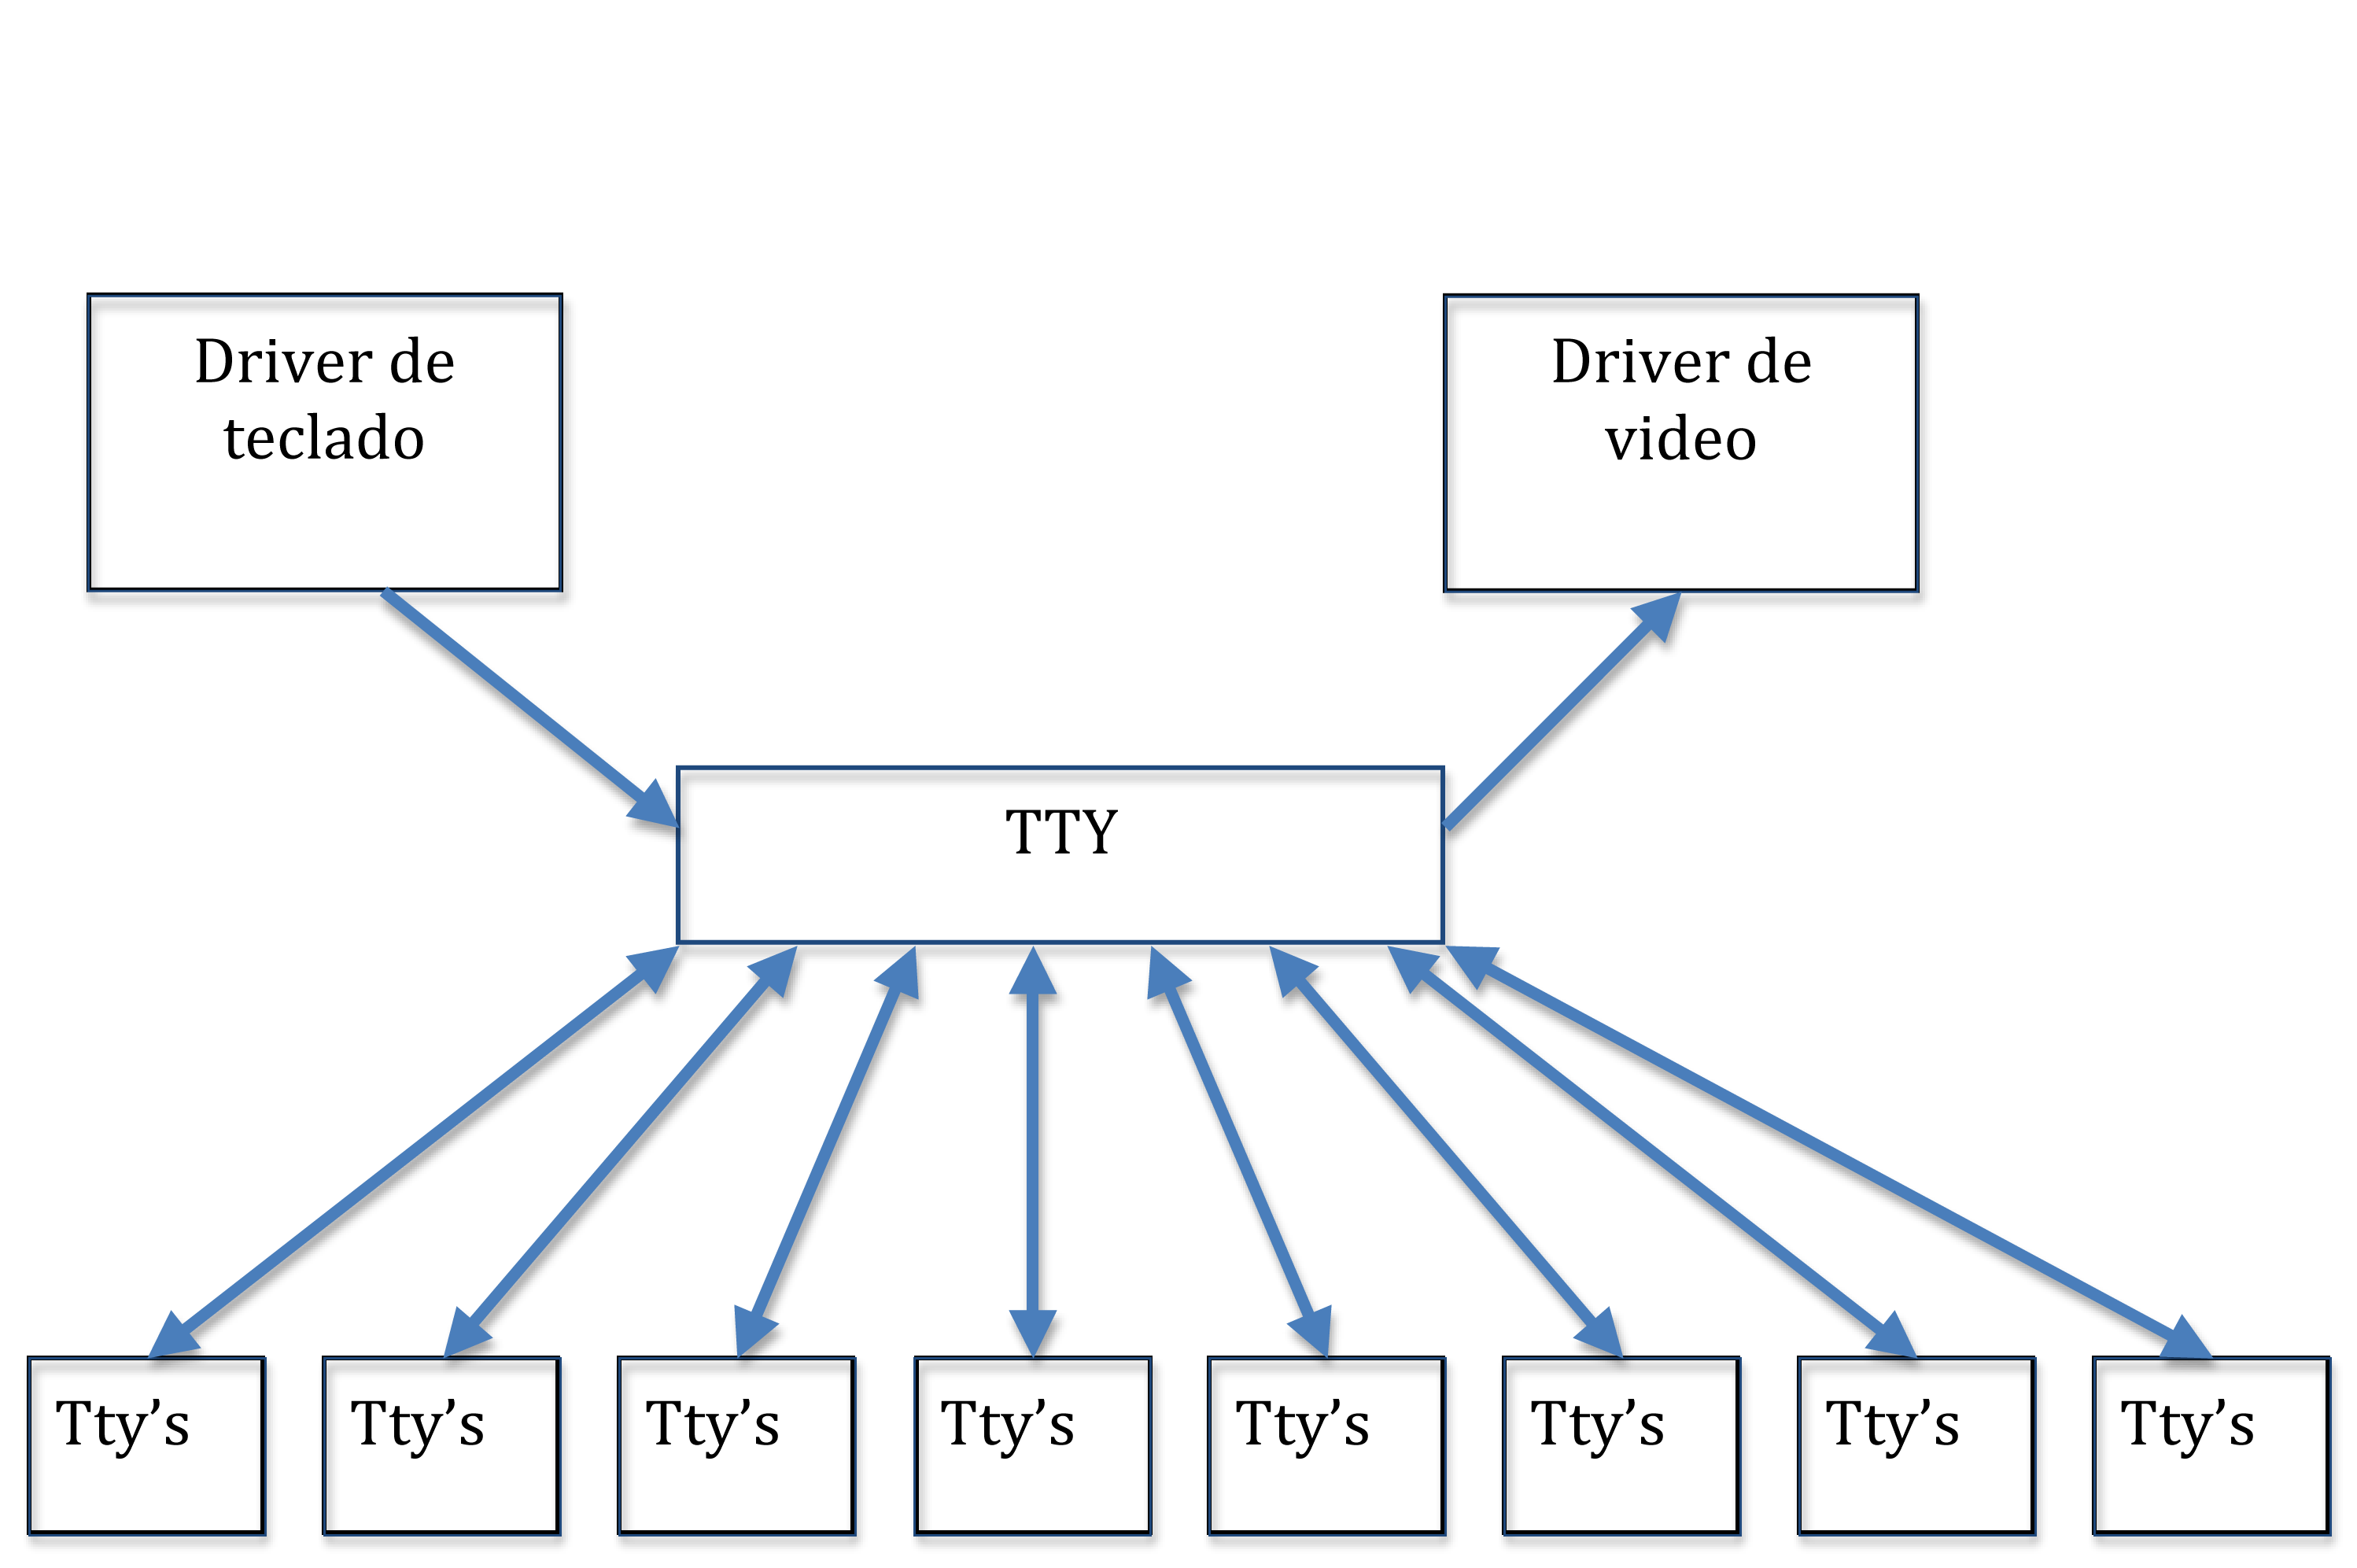
\includegraphics[angle=0, width=1\textwidth , height=0.3\textheight]{flujoTTY.png} 
	\caption{ Flujo de datos entre los driver, y la tty. }
	\end{center} 
	\end{figure}
	
	\begin{figure}
	\begin{center} 
	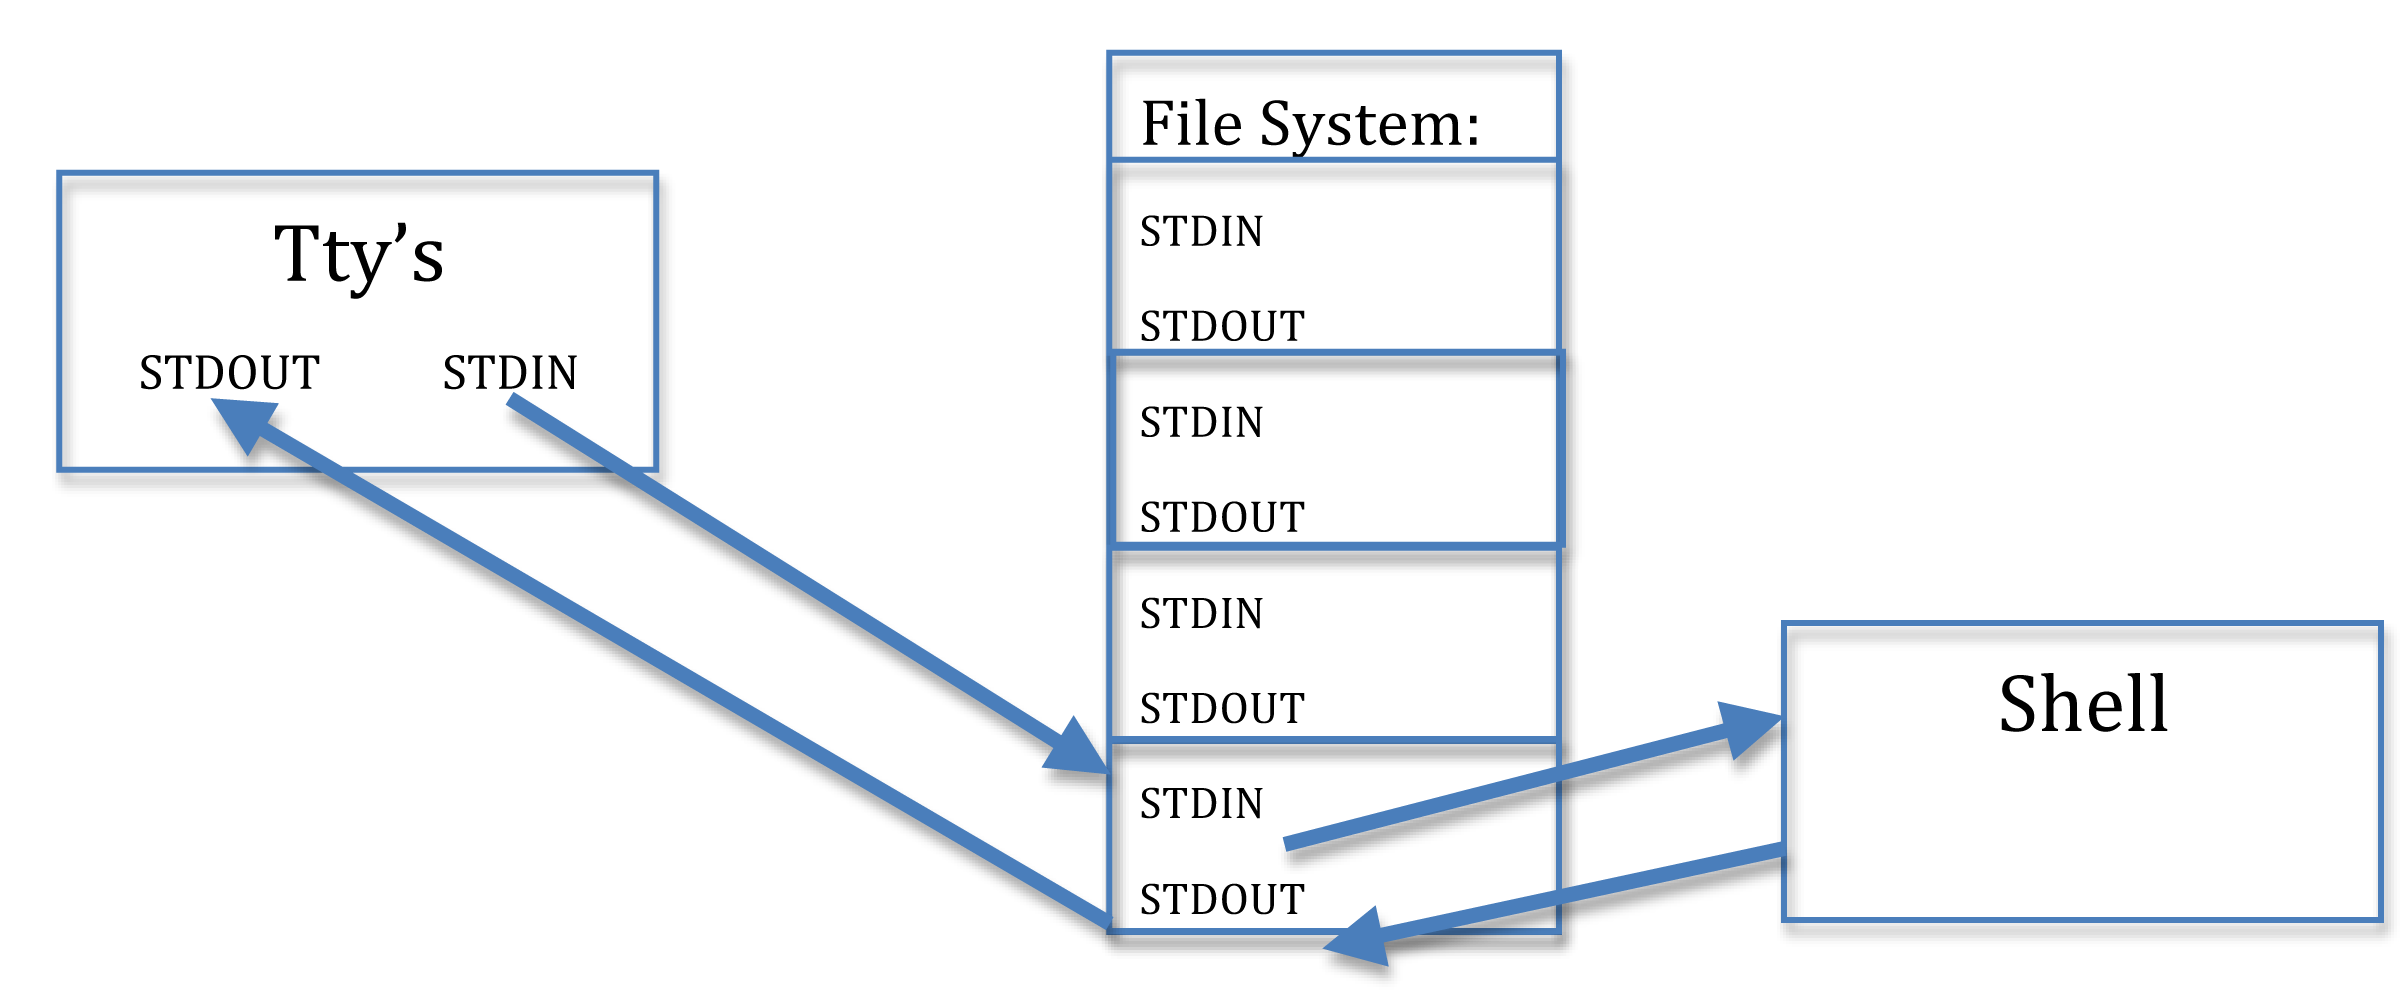
\includegraphics[angle=0, width=1\textwidth , height=0.3\textheight]{flujoTTY2.png} 
	\caption{Flugo de datos entre los procesos, la tty y el stdout}
	\end{center} 
	\end{figure}

	\subsection{Problemas y soluciones}
		Se obtuvieron muchos problemas con la TTY ya que a medida que se iba leyendo caracteres o preguntando algo, nos dabamos cuenta que teniamos que mejorarlo por lo tanto, las TTYs sufieron muchos cambios.\\
		El primer problema que nos surg\'io fue el tema de los lenguajes que manejaba la TTY, el tema de los buffers. En un principio teniamos un \'unico \textit{STDIN}, por lo que tuvimos que cambiarlo y asignarles un buffer \textit{STDIN} a cada TTY. \\
		Otro problema con esto fue la diferenciaci\'on entre el \textit{STDIN} y \textit{stdin}, donde para nosotros el \textit{stdin} es la entrada est\'andar del proceso que estaba corriendo y no necesariamente es el que esta en foco en la TTY actual, menos aun podria serlo si es una shell que esta dormida. Por lo tanto se tuvieron que modificar los write y read para escriban sobre un \textit{stdin} y \textit{stdout} indicado.
		Un problema de no gran envergadura fue el manejo de los indices, ya que en un principio se utiliz\'o dos variables de desplazamiento unicamente y se incrementaba de a un paso o en el caso que fuese un caracter de control se desplazaba lo indicado por ese caracter, pero por cuestiones de simplicidad se decidi\'o utilizar una varible que me indica la cantidad de caracteres que escribi\'o en el \textit{STDOUT} de la TTY, una variable que me dice la fila en la cual se encuentra y una variable para la columna. Del mismo modo para las variables de lectura, se siguio el mismo criterio.
	\subsection{Limitaciones}
		Se tuvieron que tomar siertas consideraciones para poder desarrollar el sistema, una de ellas es , una limitada catidad de caracteres que se pueden lamacenar en modo Raw, debido a que si no se presiona \textbf{new line}, el buffer de la tty no es refresacado, por esa razon se perderian los caracteres ingresados una vez que el buffer este completo.
\section{Procesos}
	\subsection{Objetivo}
	Se lanzaran inicialmente nueve procesos, y seran creados en el siguiente orden, init, shell1, shell2, ... ,shell8. En la figura 3, se presentan un diagrama de arbol, demostrando la relacion entre ellos. Al comenzar a correr init se dureme en espera del retorno de sus hijos. Por otrolado las shells son bloquedas por un getchar.
	\subsection{Modelado}
	A diferecncia de linux, los procesos corren el mismo archivo binario, por esa razon se debe tener mucho cuidado con las variables globales. Cada proceso al ser creado obtiene un frame , que luego sera utilizado como heap. 
	\subsection{Esquema general}
	A continuaci\'on en la figura 3,  se muestra un diagrama del estado inicial del sistema una vez completada la inicializaci\'on. En la figura 4, se puede ver que pasaria si el usuario quiesiera ejecutar el proceso top.
	
		\begin{figure}
	\begin{center} 
	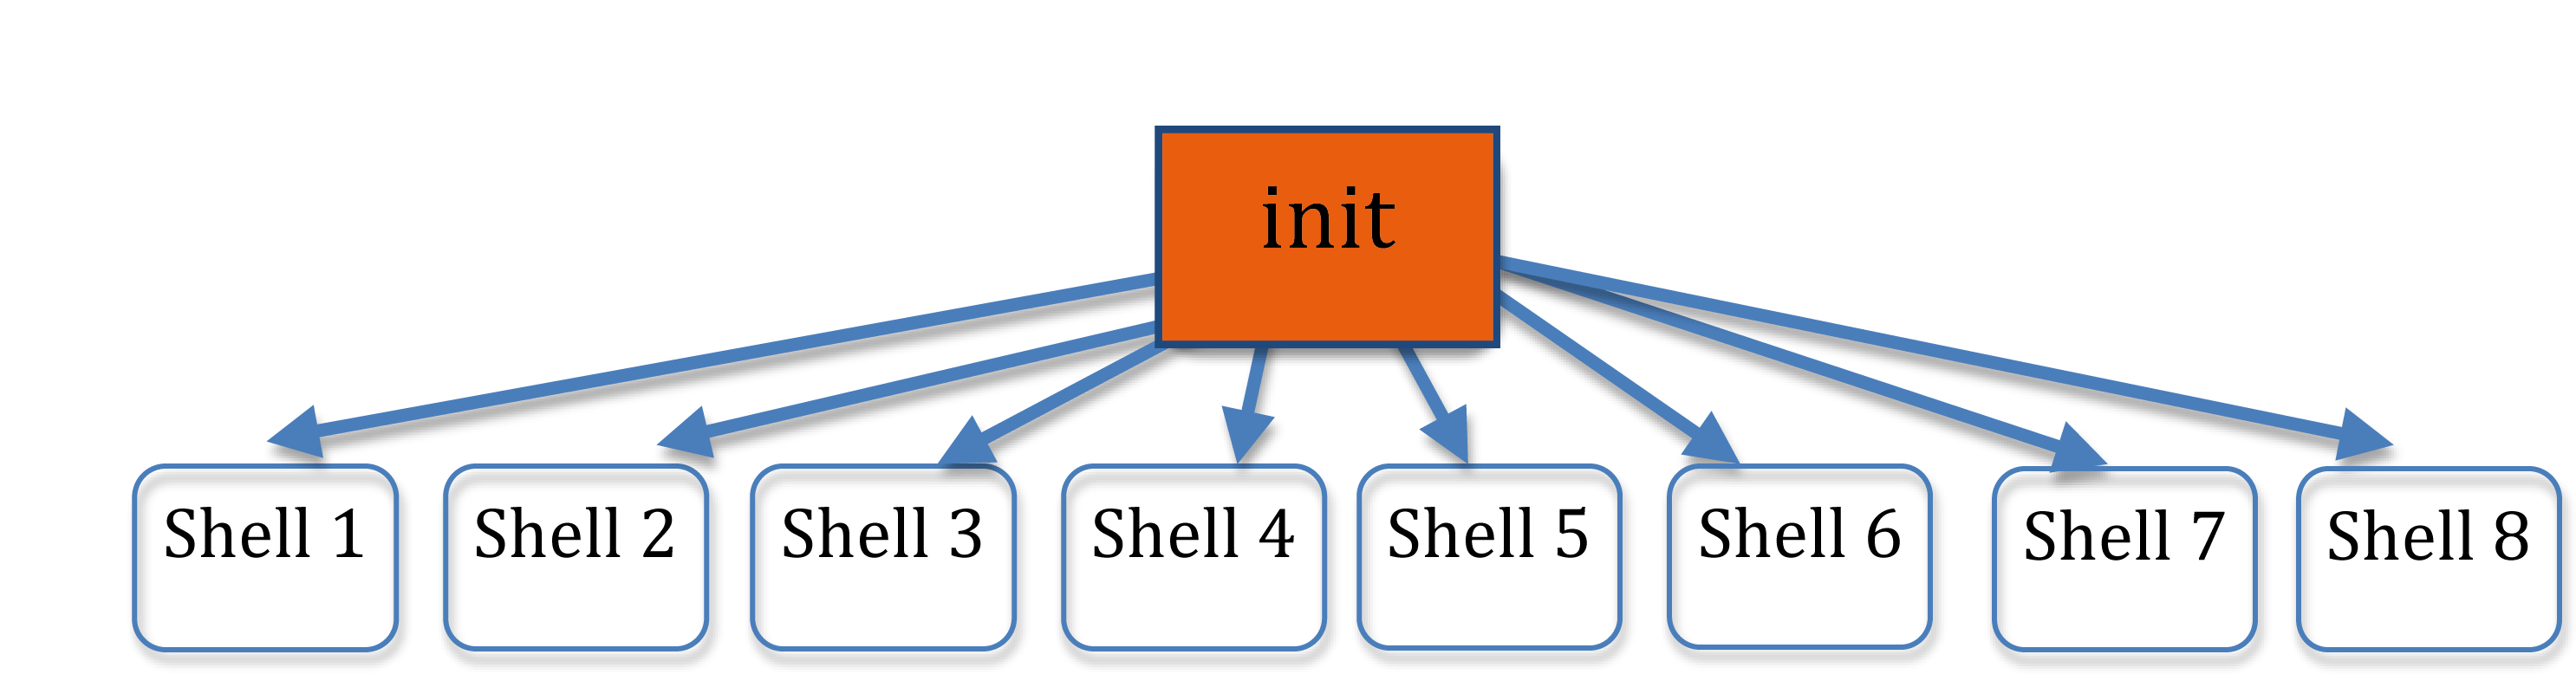
\includegraphics[angle=0, width=1\textwidth ]{procesos.png} 
	\caption{ Estado inicial del sistema, los proceso que estan en azul estan blockeados, y los que estan en naraja esperan a que termines sus hijos. El sentido de las flechas define a quien se esta esperando }
	\end{center} 
	\end{figure}
	
	\begin{figure}
	\begin{center} 
	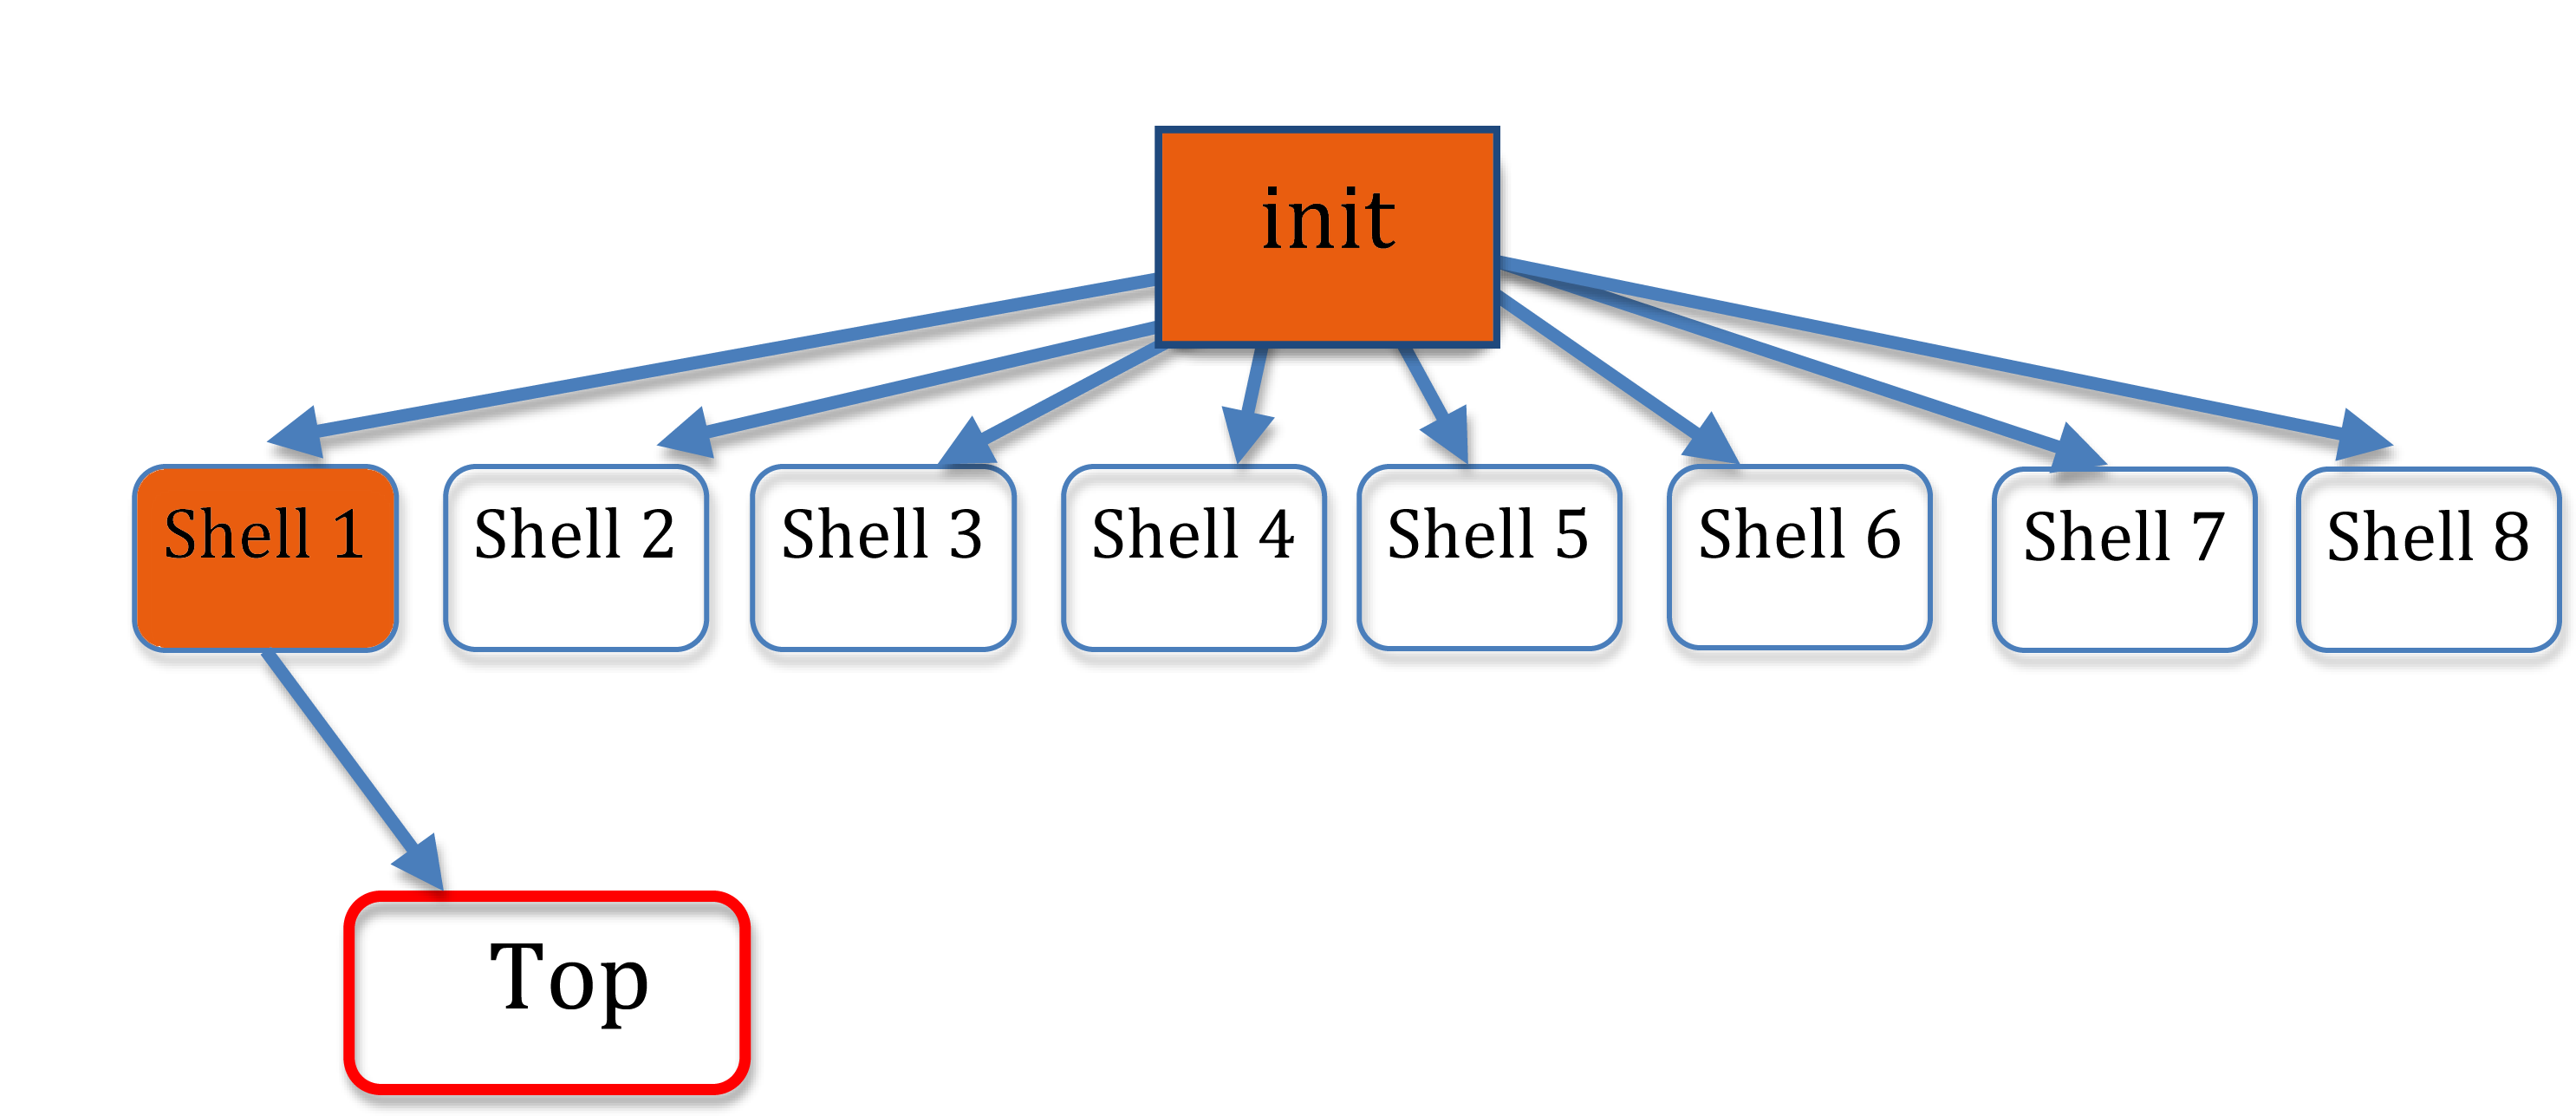
\includegraphics[angle=0, width=1\textwidth ]{proceso2.png} 
	\caption{Estado inicial del sistema, los proceso que estan en azul estan blockeados, y los que estan en naraja esperan a que termines sus hijos, y rojo el proceso que se esta ejecutando. El sentido de las flechas define a quien se esta esperando}
	\end{center} 
	\end{figure}

	\subsection{Creacion de procesos}
	\subsection{Herencia de TTY's}
	\subsection{Muerte de un proceso}
	\subsection{Procesos ejecutados en background}
	\subsection{Procesos especiales}
	\subsubsection{Top}
	\subsubsection{Shell}
	En esta secci\'on se hablara acerca de como fue adaptada la shell para poder funcionar en un sistema multi tarea. \\ 
	Como la shell que se tomo como base fue dise\~nada para correr en un sistema multi tarea, se tuvieron que realizar ciertas adaptciones. Una de ellas fue, que las variables globales deberian pertenecer solamente a esa shell, por esa razon se realizo un vector donde sfueron almacenadas estruras con todos los datos pertinentes para el correcto funcionamiento de la shell. Cada shell almacenaba en su heap dichas estructuras, esto asegura un nivel mas de seguridad, ya que una shell no podra acceder a datos de otra, por que no estarina presentes las paginas. \\
	En la misma se colocaron proceso de pruba que se pueden ejecutar para probar la funcionalidad del sistema.

	\subsection{Problemas y soluciones}
	\subsection{Limitaciones}
	


\section{Multitasker}
	\subsection{Objetivo}
	Intercambiar tareas mediante software, y una correcta construcci\'ion del stack frame.
	\subsection{Modelo}
	\subsection{Esquema general}
	\subsection{Problemas y soluciones}
	\subsection{Limitaciones}

\section{Scheduler}
	\subsection{RPG}
	\subsubsection{Modelo}
		Implementar un algoritmo basado en juegos RPG. El algoritmo consite en asignarle un puntaje a un proceso en cada llamado del scheduler. Cuando un proceso llega al puntaje designado como m\'aximo se lo agrega a la lista de procesos listos para ejecutar. Luego se verifica que proceso es el que tiene mas antiguedad. Una vez devuelto el proceso a procesar, se reinicia el contador de puntos rpg y la antiguedad.
	\subsubsection{Problemas y soluciones}
		Principalmente tuvimos un problema manejando la antiguedad de los procesos, luego decidimos tomar una funci\'on de evaluaci\'on que nos permite ir pasando por todos los procesos, que no alcanzen inmediatamente el puntaje m\'aximo de rpg, para luego ser atendido.
	\subsubsection{Limitaciones}
		La funci\'on de evaluaci\'on en el caso de que se aumente la cantidad de procesos o disminuya habria que cambiarla, porque es en funci\'on de prioridades y cantidad m\'axima de procesos, tambien habria que modificar el puntaje m\'aximo de rpg a alcanzar

\subsection{Round-Robin}
	\subsubsection{Objetivo}
		Implementar un algoritmo del tipo Round Robin. Basicamente se comporta como una lista circular donde se van devolviendo todos los procesos que esten en estado \textbf{READY} en el orden que se encuentran en la tabla de procesos.
	\subsubsection{Modelo}
		El modelo tomado es el siguiente, en el que la gran mayor\'ia debe utilizar. Se toma la lista de procesos y se la recorre en forma lineal verificando si algun proceso se encuentra listo para ser atendido, en el caso de que haya alguno se lo devuelvo y en la pr\'oxima llamada se arranca a recorrer desde esa posicion y se realiza el mismo recorrido ya explicado anteriormente.
	\subsubsection{Problemas y soluciones}
		En un principio el algoritmo se quedaba en un loop infinito ya que buscasa desde init y como siempre estaba listo lo devolvia y a veces no retornaba o era interrumpido. Por lo tanto una soluci\'on fue llamar al scheduler en caso de que haya algun proceso para correr distinto de init. En un principio teniamos problemas con el algoritmo porque compilabamos con la opci\'on de optimizaci\'on y se agregaban funciones en el c\'odigo que no queriamos, luego de darnos cuenta de ese error comenz\'o a andar el algoritmo.
	\subsubsection{Limitaciones}
		El algoritmo en si no maneja el tema de prioridades, sino en el orden el cual fueron creados los procesos. Se podria hacer que la creaci\'on de procesos los inserte en forma ordenada en la tabla de procesos por lo tanto el algortimo \textit{Round Robin} de alguna forma estar\'ia teniendo en cuenta el tema de prioridades.

\subsection{IPCs Implementaciones}
	\subsubsection{Shared memory}
		Se implement\'o un IPC basado en Shared memory, donde la cantidad de shared memory esta definida por un define. Se decidi\'o utilizar la estructura que utiliza System Five para la shared memory y Posix para los sem\'aforos. Cada shared memory ya tiene asociado un sem\'aforo y la cantidad de frames que tiene desiganados para utilizar.
	\subsubsection{Objetivo}
		Implementar un juego en donde se pueda verificar la comunicaci\'on entre los dos procesos mediante un IPC, en nuestro caso \textbf{Shared Memory}.
	\subsubsection{Modelo}
		En un principio se decidi\'o implementar como juego un Chat entre varias shells, pero finalmente se eligi\'o hacer la batalla naval con cierta restricciones. La creaci\'on de barcos se genera en forma aleatoria, es decir que se implement\'o un random muy b\'asico donde usa un polinomio de grado 1 y como semilla utiliza los tick realizados por el timer tick hasta el momento. El juego es de dos personas unicamente, como la tradicional batalla naval.
	\subsubsection{Esquema general}
		La forma que se nos ocurrio para comunicar los dos procesos es que cuando crea ese procesa el juego te da la opci\'on de ser host o unirte a una partida ya creada. Por lo tanto cuando creo el primer proceso puedo elegir entre ser host o unirme a una partida ya creada, la forma de unirse es que el host cuando crea se le muestra en pantalla el ID de la shared memory creada, por lo tanto el jugador 2 debe ingresar ese id para unirse a esa partida. Una vez ya pasados los primeros pasos comienza el juego. La comunicaci\'on que viaja por la shared memory son las posiciones del tablero en donde se ubicaron las bombas. En un principio se habia dicho de poner el tablero de cada jugador en la shared memory y que el jugador escriba directamente sobre esa posicion, pero nos dimos cuenta que en verdad la informaci\'on que necesitan los dos son las posiciones del tablero para cada uno actualizar donde fue puesta la bomba y verificar si le dio a algun barco o si fue agua. \\
		Cada vez que un usuario ingresa una posici\'on en donde desea ubicar la bomba se bloquea el tablero y una vez enviado el mensaje se desbloquea. De esta forma evitamos que los dos jugadores pongan en el mismo instante dos posiciones distintas y se mezclen sus ubicaciones.
	\subsubsection{Problemas y limitaciones}
		Un problema fue tomar la decisi\'on de ubicar los barcos, si el usuario los podia ubicar o si lo generabamos nosotros, se opto por la segunda y los barcos pueden estar unicamente verticales y horizontales, no diagonales. \\
		Otro problema que nos surgio fue que los sem\'aforos se quedaban esperando pero se seguia imprimiendo el tablero esperando la conexi\'on de algun usuario al juego, por lo tanto decidimos modificar los sem\'aforos para que se queden esperando y no pueda realizar otra cosa, entonces cuando alguien ingresa una posici\'on se refresca el tablero.  

\subsection{Conclusi\'on}
Fue de mayor importancia, seguir algunas convenciones de unix, ya que se facilito el dise\~no del proyecto en general. Por ortro lado es bastante complejo adaptar un sistema mono tarea a multi tarea como tuvimos que hacer, debido a esto genero problemas serios en el desarrolo del trabajo, mas que nada en las ultimas etapas. Se quiere resaltar que si  no se toman desiciones correctas en la etapa de dise\~no del proyecto, se puede llegar aun punto en donde no se tenga otra solucion que tener que realizar una restructuracion importante. Por esta razon se decidio como se dijo anteriormente aplicar a grandes rasgos las estrucutara que utiliza unix.\\
Se opto por un kernel monolitico, por una cuestion de eficiencia, y codificacion simple. El cambio de contexto resulto muy complejo, ya que este implica una precicion a la que no estabamos acostumbrados. Se hace incapie en este tema mas que nada en la cosntrucci\'on del stackframe.\\
A diferencia de proyectos anteriores, se realizo una programci\' on en parejas, ya que se necesitaba una atencion constante. Se pudo optar por esta metodologia por que el codigo no era extenso, sino que complejo.\\
Al momento de desarrollar el juego se decidio buscar un juego y adaptarlo a las necesidades, ya que el trabajo no estaba apuntado a esa tarea.\\
Se pudieron afianzar conocimientos sobre la estructura y la funcionalidad de un sistema operativo,  creacion de procesos  y cambios de contexto. Quedo en evidencia la razon de muchas deciciones que toman los sistemas , cuando estos estan en etapa de desarrolo.\\ 


\subsection{Bibliograf'ia y fuentes}

\end{document}